% Configurazione
\documentclass[12pt, a4paper]{report}

\usepackage{graphicx}
\usepackage[table,xcdraw]{xcolor}
%\usepackage{xcolor}
\usepackage{titlesec}
\usepackage{siunitx}
\usepackage{float}
\usepackage[italian]{babel}
\usepackage{array}
\newcolumntype{L}[1]{>{\raggedright\arraybackslash}p{#1}}
\newcolumntype{C}[1]{>{\centering\arraybackslash}p{#1}}
\newcolumntype{R}[1]{>{\raggedleft\arraybackslash}p{#1}}

\usepackage{hyperref}
\hypersetup{
    colorlinks,
    linkcolor=black,
    urlcolor=blue
}

\graphicspath{ {immagini/} }
\definecolor{RossoUnipd}{HTML}{B5121B}
\titleformat{\chapter}{\normalfont\huge}{\thechapter.}{20pt}{\huge\textbf}

% Variabili
\newcommand{\titolo}{Piano di Progetto}



% Struttura
\begin{document}
  \begin{minipage}[]{0.3\textwidth}
  
\includegraphics[width=0.7\textwidth]{logo_uni}
\end{minipage}
\begin{minipage}[]{0.6\textwidth}
  \textcolor{RossoUnipd}{
    \textbf{Università degli Studi di Padova} \\
    Laurea: Informatica \\
    Corso: Ingegneria del Software \\
    Anno Accademico: 2021/2022
  }
\end{minipage}

\bigskip

\begin{minipage}[]{0.3\textwidth}
  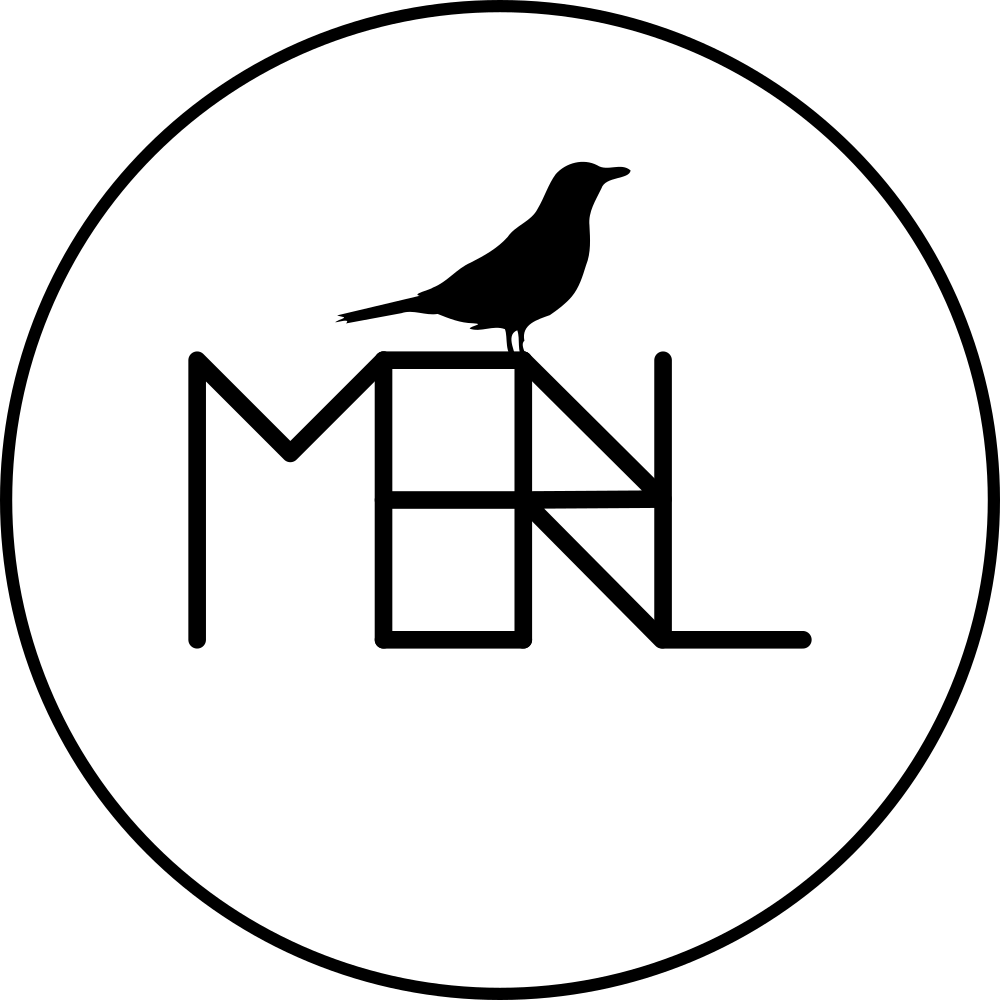
\includegraphics[width=0.7\textwidth]{logo_merl}
\end{minipage}
\begin{minipage}[]{0.6\textwidth}
  Gruppo: MERL \\
  Email: \texttt{merlunipd@gmail.com}
\end{minipage}

\bigskip
\bigskip
\bigskip

  \begin{center}
  \Huge\textbf{\titolo}
\end{center}

\bigskip
\bigskip
\bigskip
  \newpage
  \begin{center}
  \huge{Registro delle Modifiche}
\end{center}
\newcommand{\aCapo}[1]{%
  \begin{tabular}{@{}c@{}}\strut#1\strut\end{tabular}%
}
\begin{center}
  \begin{tabular}{|p{2cm}|p{2cm}|p{4cm}|p{5cm}|}
    \hline
    \textbf{Versione} & \textbf{Data} & \textbf{Autore/Verificatore} & \textbf{Modifica}                    \\ \hline
    v0.1.4            & 15/01/2022    & \aCapo{Marco Mamprin\\Mattia Zanellato} & Aggiunte sottosezione "Testing"  \\ \hline  
    v0.1.3            & 09/01/2022    & \aCapo{Marco Mamprin\\Emanuele Pase} & Aggiunte sottosezione "Metriche"  \\ \hline           
    v0.1.2            & 07/01/2022    & \aCapo{Riccardo Contin\\Marko Vukovic} & Aggiunte sottosezioni "Preventivo" e "Consuntivo"  \\ \hline
    v0.1.1            & 02/01/2022    & \aCapo{Marko Vukovic\\Emanuele Pase} & Aggiunta sezione automazione  \\ \hline
    v0.1.0            & 27/12/2021    & Riccardo Contin & Approvazione  \\ \hline
    v0.0.13           & 24/12/2021    & \aCapo{Emanuele Pase\\Marco Mamprin} & Fix minori  \\ \hline
    v0.0.12           & 24/12/2021    & \aCapo{Lorenzo Onelia\\Emanuele Pase} & Fix minori \\ \hline
    v0.0.11           & 21/12/2021    & \aCapo{Marko Vukovic\\Marco Mazzucato} & Aggiunta sezione "Gestione dei Processi Organizzativi" \\ \hline
    v0.0.10            & 18/12/2021    & \aCapo{Emanuele Pase\\Marco Mazzucato} & Aggiunta sezione "Sviluppo" \\ \hline
    v0.0.9            & 17/12/2021    & \aCapo{Mattia Zanellato\\Lorenzo Onelia} & Aggiunta sezione "Fornitura" \\ \hline
    v0.0.8            & 17/12/2021    & \aCapo{Mattia Zanellato\\Lorenzo Onelia} & Aggiunto capitolo "Introduzione" \\ \hline
    v0.0.7            & 16/12/2021    & \aCapo{Marco Mazzucato\\Marco Mamprin} & Aggiunta sezione "Documentazione" \\ \hline
    v0.0.6            & 14/12/2021    & \aCapo{Marco Mamprin\\Riccardo Contin} & Aggiunta sezione "Formazione" \\ \hline
    v0.0.5            & 14/12/2021    & \aCapo{Marco Mamprin\\Riccardo Contin}   & Aggiunta sezione "Validazione" \\ \hline
    v0.0.4            & 14/12/2021    & \aCapo{Marco Mamprin\\Riccardo Contin}   & Aggiunta sezione "Gestione della Qualità" \\ \hline
    v0.0.3            & 11/12/2021    & \aCapo{Lorenzo Onelia\\Emanuele Pase} & Aggiunta sezione "Verifica" \\ \hline
    v0.0.2            & 10/12/2021    & \aCapo{Emanuele Pase\\Riccardo Contin}  & Aggiunta sezione "Gestione della configurazione" \\ \hline
    v0.0.1            & 08/12/2021    & \aCapo{Marko Vukovic\\Marco Mazzucato}   & Aggiunta sezione "Infrastruttura" \\ \hline
    v0.0.0            & 07/12/2021    & \aCapo{Marko Vukovic\\Marco Mazzucato}   & Creata prima struttura del documento \\ \hline
  \end{tabular}
\end{center}

  \tableofcontents

  % Capitoli
  \chapter{Introduzione}

\section{Scopo del documento}

Il \textit{Piano di Progetto} è un documento di fondamentale importanza per riuscire a lavorare nel migliore dei
modi. La sua struttura è:
\begin{itemize}
    \item \textbf{Analisi dei rischi: } permette di indicare i possibili rischi, la probabilità che essi si verifichino e la loro gravità;
    \item \textbf{Pianificazione: } permette di pianificare le milestone;
    \item \textbf{Preventivo: } permette di indicare le ore e i costi che si intende impiegare in ogni periodo pianificato;
    \item \textbf{Consuntivo: } permette di analizzare il reale svolgimento dei periodi passati rispetto a com'erano stati preventivati;
    \item \textbf{Mitigazione dei rischi: } permette di analizzare i rischi che si sono effettivamente verificati. 
\end{itemize}

\section{Glossario}

Nel caso ci fossero termini che provocano difficoltà di interpretazione o che risultano ambigui, esiste un \textit{Glossario}
che contiene una serie di termini con relativa descrizione che fornisce un supporto alla consultazione del documento.

\section{Riferimenti}
\subsection{Riferimenti normativi}
\begin{itemize}
  \item \textit{Norme di Progetto}
  \item Capitolato d'appalto C5 - Zucchetti S.p.A.: Login Warrior \\
  \url{https://www.math.unipd.it/~tullio/IS-1/2021/Progetto/C5.pdf}
\end{itemize}

\subsection{Riferimenti informativi}
\begin{itemize}
  \item Slide T5 - Corso di Ingegneria del Software - Il ciclo di vita del SW \\
  \url{https://www.math.unipd.it/~tullio/IS-1/2021/Dispense/T05.pdf}
  \item Slide T6 - Corso di Ingegneria del Software - Gestione di progetto \\
  \url{https://www.math.unipd.it/~tullio/IS-1/2021/Dispense/T06.pdf}
\end{itemize}

  \chapter{Modello di sviluppo}


\section{Modello incrementale}
  \chapter{Analisi dei rischi}

%valutare quali sezioni inserire in base ai documenti passati
  \chapter{Pianificazione}

Scadenze:
\begin{itemize}
    \item RTB (Requirements and Technology Baseline) : 25/02/2022;
    \item PB (Product Baseline) : 05/04/2022;
    \item CA (Customer Acceptance) : 06/05/2022.
\end{itemize}

\section{Verso la RTB}

\textit{Periodo: 29/11/2021 - 24/02/2021}

\subsection{Primo periodo}

\textit{Periodo: 29/11/2021 - 18/12/2021}

In questa prima fase risulta di priorità massima discutere tutte le regole già introdotte
e applicate nello svolgimento del progetto che però non sono ancora state documentate.
Questo per avere un documento scritto a disposizione di tutti i membri che consenta di
non avere dubbi su come svolgere qualsiasi attività e su come utilizzare le risorse.
\par In questa fase è importante anche individuare tutti i vari rischi che possono portare
problemi allo svolgimento del progetto per non essere colti di sorpresa.
\par Di fondamentale importanza è anche iniziare a pianificare le prime attività e quindi
le prime milestone in modo da organizzare le risorse e di fornire un preventivo. 

\begin{figure}[!ht]
    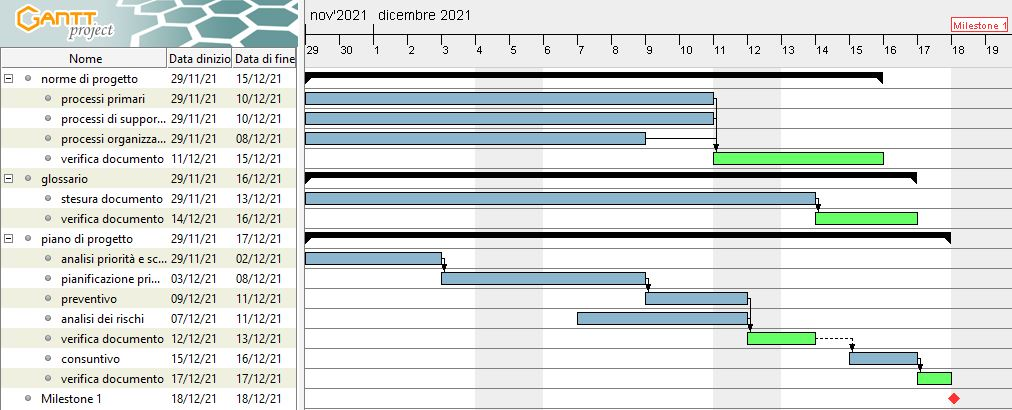
\includegraphics[width=1.0\textwidth]{Gantt1}
    \caption{Diagramma di Gantt della prima milestone} 
\end{figure}

\newpage

\subsection{Secondo periodo}

\textit{Periodo: 20/12/2021 - 10/01/2022}

In questa fase diventa importante analizzare nel dettaglio il capitolato per riuscire a
cogliere i casi d'uso necessari. Inoltre, per evitare dubbi e per non effettuare
scelte sbagliate, sarà opportuno organizzare uno o più incontri con il proponente in modo da
condividere idee e dubbi sorti durante l'analisi che sarà sicuramente più approfondita di quella
effettuata durante la scelta del capitolato.
\par Da tutto ciò si inizierà a redarre l'\textit{Analisi dei Requisiti}, documento importantissimo per il progetto poiché
conterrà tutti i casi d'uso individuati, i requisiti obbligatori, quelli desiderabili e quelli opzionali.
\par In questa fase è opportuno stilare anche il Piano di Qualifica, necessario per individuare
i metodi per garantire la qualità di processo e di prodotto.

\begin{figure}[!ht]
    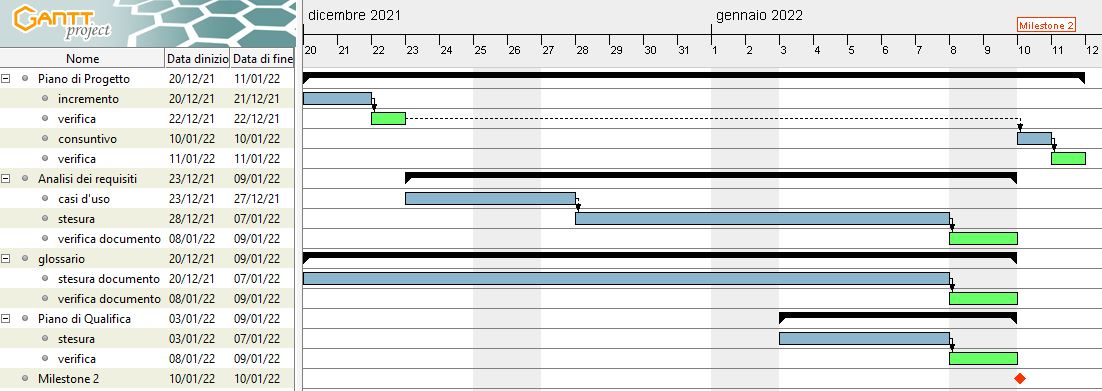
\includegraphics[width=1.0\textwidth]{Gantt2}
    \caption{Diagramma di Gantt della seconda milestone} 
\end{figure}

\subsection{Terzo periodo}

\textit{Periodo: 15/01/2022 - 04/02/2022}

Dopo avere avuto un colloquio con il proponente sui casi d'uso e i requisiti è importante progredire con
l'\textit{Analisi dei Requisiti}. Diventa, poi, fondamentale studiare le tecnologie e gli strumenti necessari
per realizzare il prodotto. Questo permetterà di realizzare il PoC (Proof of Concept), una versione semplificata 
del prodotto finale che permetta di intuire se la direzione è quella giusta e che mostri al proponente se lo 
sviluppo è corretto.

\begin{figure}[!ht]
    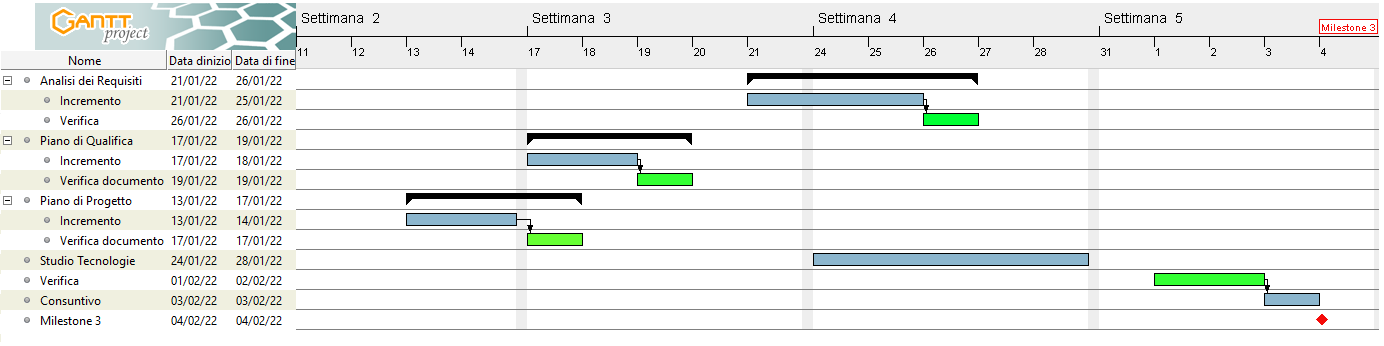
\includegraphics[width=1.0\textwidth]{Gantt3}
    \caption{Diagramma di Gantt della terza milestone} 
\end{figure}


\subsection{Quarto periodo}
\textit{Periodo: 7/02/2022 - 24/02/2022}

In quest'ultimo periodo diventa di fondamentale importanza la progettazione e la realizzazione
 del PoC. Inoltre diviene necessario il completamento e la verifica finale dei documenti prima della revisione prevista 
 per fine febbraio.


\begin{figure}[!ht]
    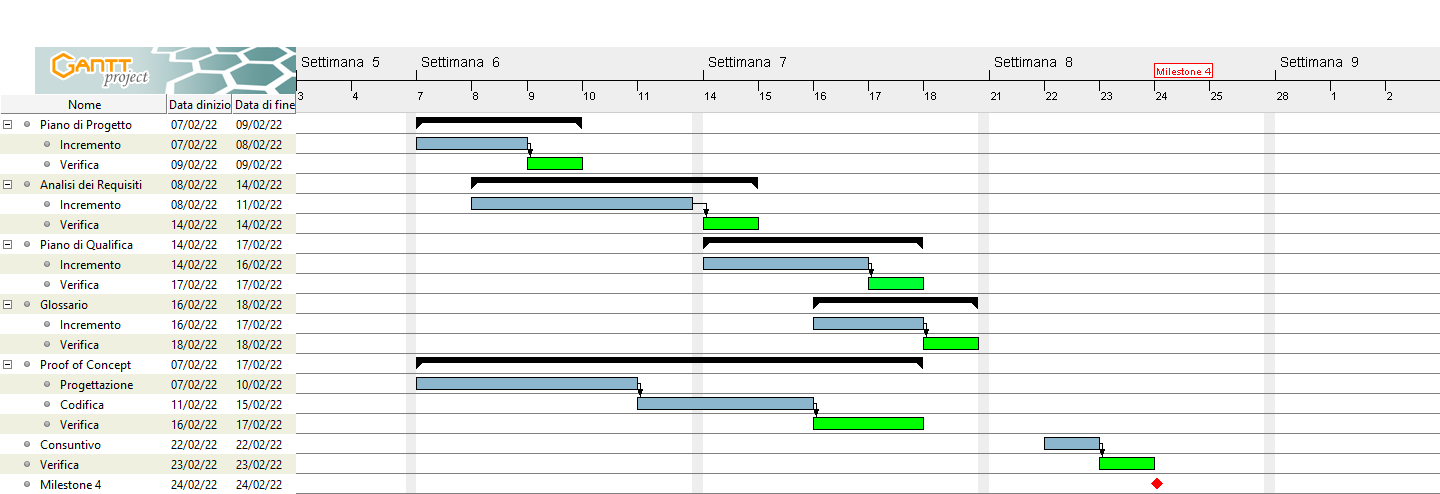
\includegraphics[width=1.0\textwidth]{Gantt4.png}
    \caption{Diagramma di Gantt della quarta milestone} 
\end{figure}

\section{Verso la PB}

\textit{Periodo: 28/02/2022 - 31/03/2022}

\section{Verso la CA}

\textit{Periodo: 04/04/2022 - 05/05/2022}
  \chapter{Preventivo}

\section{Verso la RTB}

\subsection{Primo periodo}

In questa fase i ruoli da ricoprire per portare a termine gli obiettivi
pianificati sono:
\begin{itemize}
    \item \textit{Responsabile}
    \item \textit{Amministratore}
    \item \textit{Verificatore}
\end{itemize}

\subsubsection{Preventivo orario}

\begin{table}[!ht]
    \centering
    \begin{tabular}{|l|c|c|c|c|c|c|c|}
    \hline
    \textbf{Membro} & \multicolumn{1}{l|}{\textbf{RE}} & \multicolumn{1}{l|}{\textbf{AM}} & \multicolumn{1}{l|}{\textbf{AN}} & \multicolumn{1}{l|}{\textbf{PT}} & \multicolumn{1}{l|}{\textbf{PR}} & \multicolumn{1}{l|}{\textbf{VE}} & \multicolumn{1}{l|}{\textbf{Totale ore persona}} \\ \hline
    \textit{Marco Mazzucato}  & 2 & 3  & - & - & - & 1 & 6  \\ \hline
    \textit{Marco Mamprin}    & - & 3  & - & - & - & 1 & 4  \\ \hline
    \textit{Marko Vukovic}    & 2 & 3  & - & - & - & 1 & 6  \\ \hline
    \textit{Mattia Zanellato} & - & 3  & - & - & - & 1 & 4  \\ \hline
    \textit{Emanuele Pase}    & - & 3  & - & - & - & 1 & 4  \\ \hline
    \textit{Riccardo Contin}  & - & 3  & - & - & - & 1 & 4  \\ \hline
    \textit{Lorenzo Onelia}   & - & 3  & - & - & - & 1 & 4  \\ \hline
    \textbf{Totale ore ruolo} & 4 & 21 & - & - & - & 7 & 32 \\ \hline
    \end{tabular}
    \caption{Distribuzione delle ore per la prima milestone}
\end{table}

\begin{figure}[!ht]
    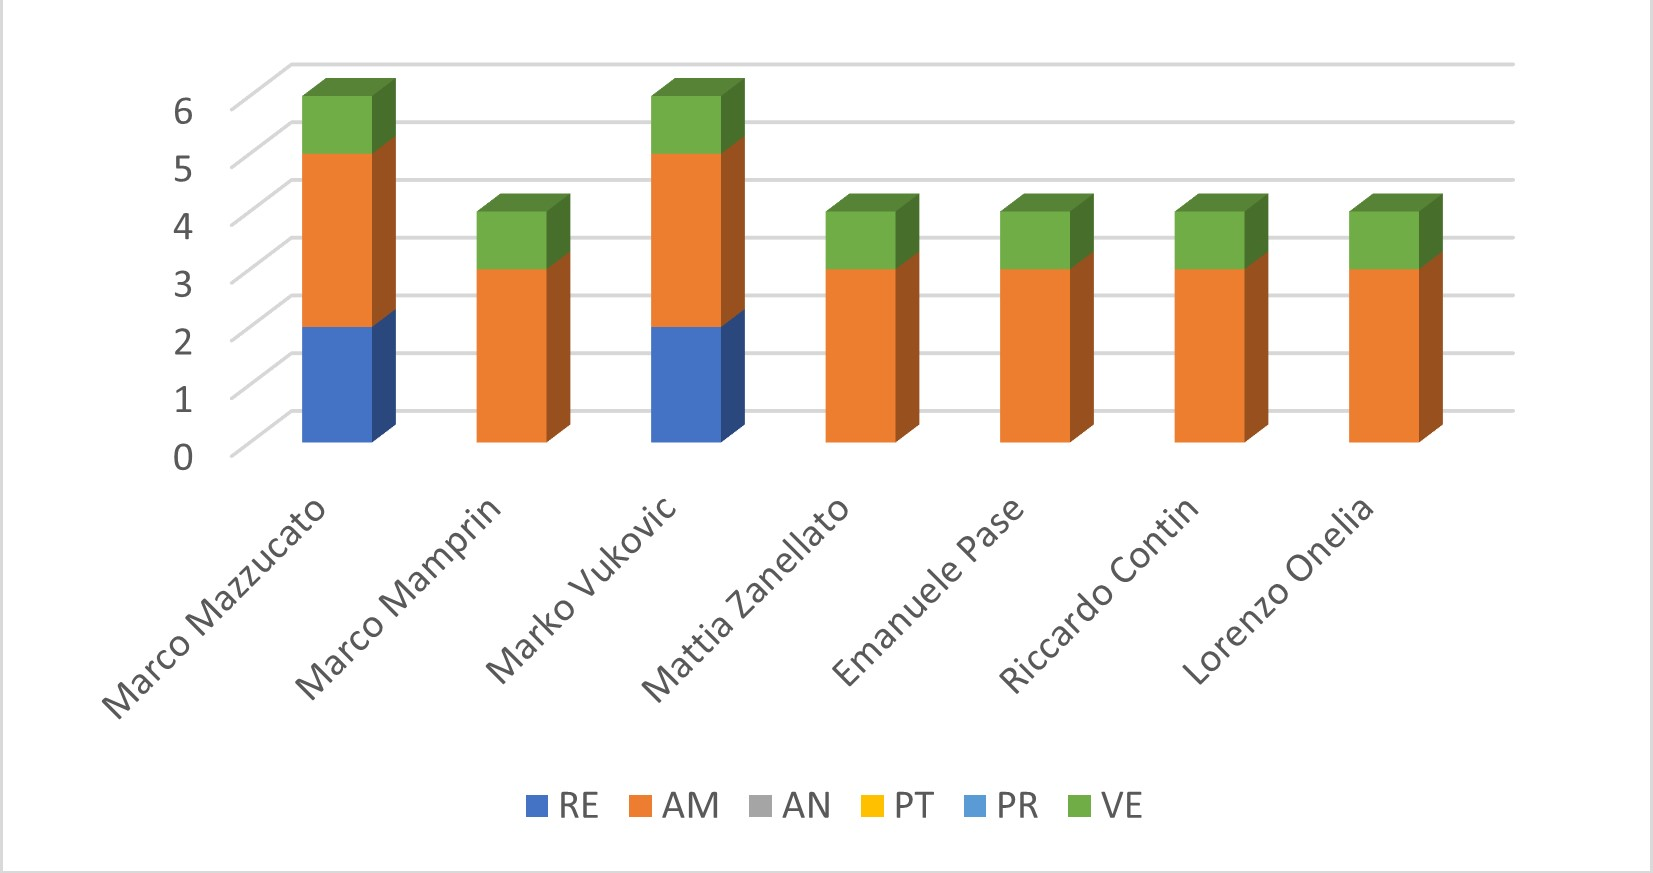
\includegraphics[width=1.0\textwidth]{Istogramma1.jpg}
    \caption{Istogramma della distribuzione delle ore} 
\end{figure}

\begin{figure}[!ht]
    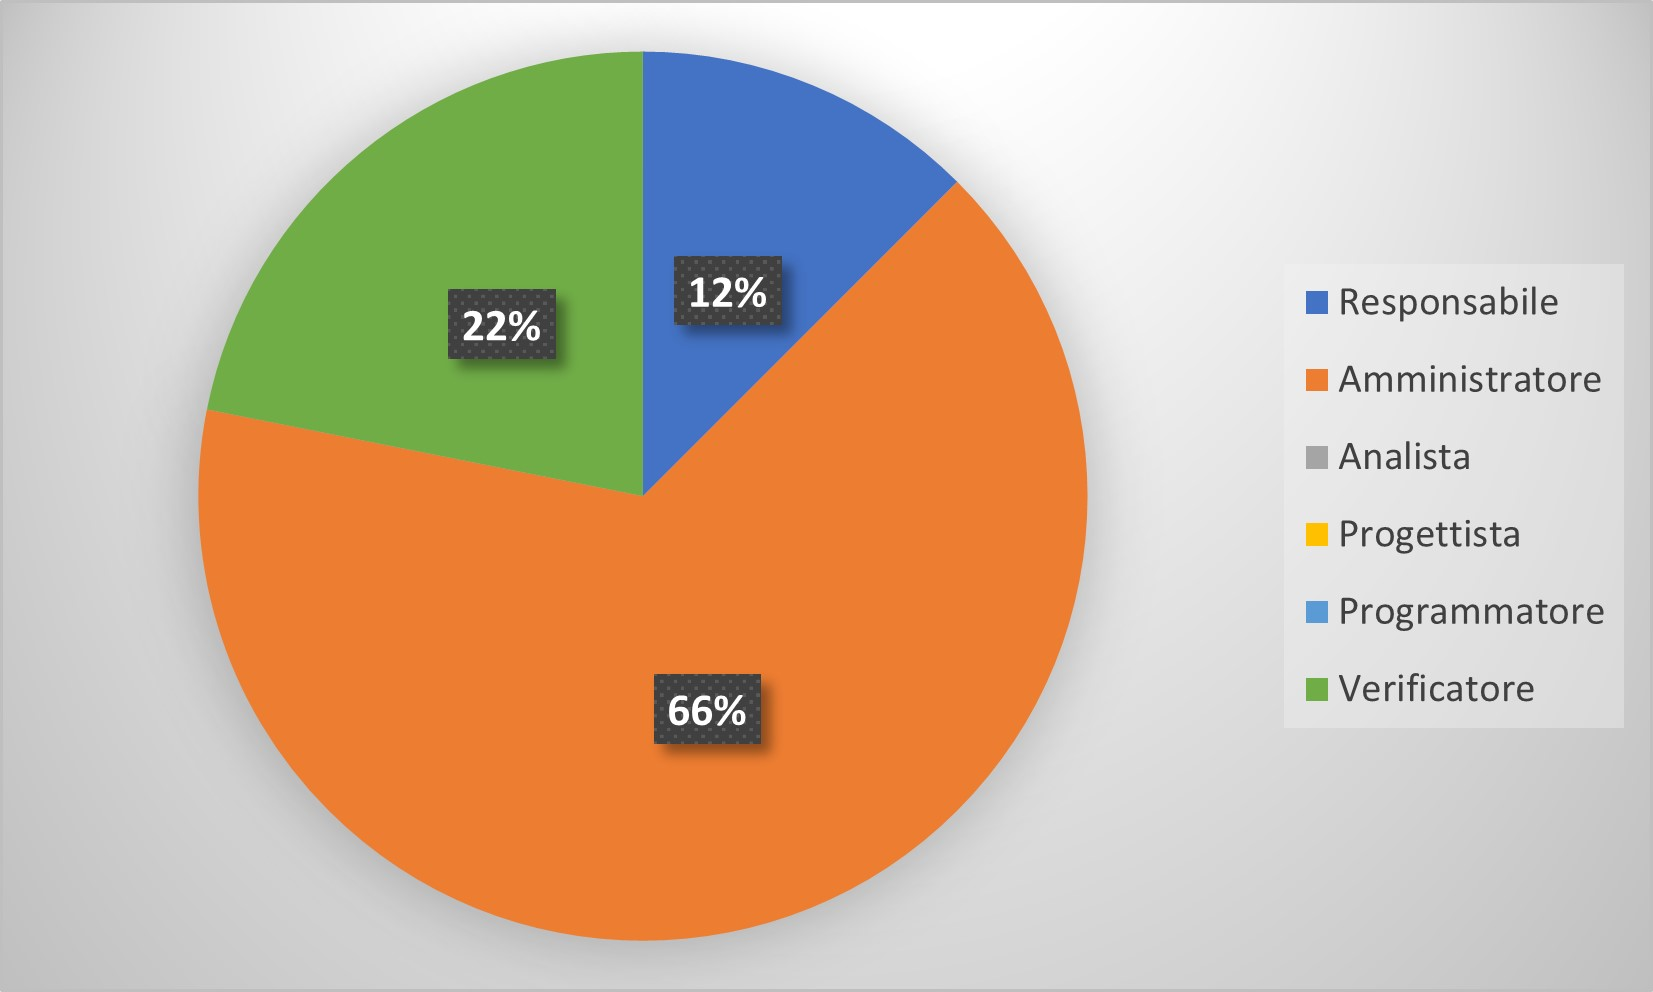
\includegraphics[width=1.0\textwidth]{Torta1.1.jpg}
    \caption{Grafico a torta della distribuzione delle ore} 
\end{figure}

\newpage
\subsubsection{Preventivo economico}

\begin{table}[!ht]
    \centering
    \begin{tabular}{|l|c|c|}
    \hline
    \textbf{Ruolo} & \multicolumn{1}{l|}{\textbf{Ore}} & \multicolumn{1}{l|}{\textbf{Costo (€)}} \\ \hline
    \textit{Responsabile} & 4 & 120 \\ \hline
    \textit{Amministratore} & 21 & 420 \\ \hline
    \textit{Analista} & - & - \\ \hline
    \textit{Progettista} & - & - \\ \hline
    \textit{Programmatore} & - & - \\ \hline
    \textit{Verificatore} & 7 & 105 \\ \hline
    \textbf{Totale} & 32 & 645 \\ \hline
    \end{tabular}
    \caption{Prospetto dei costi per la prima milestone}
\end{table}

\begin{figure}[!ht]
    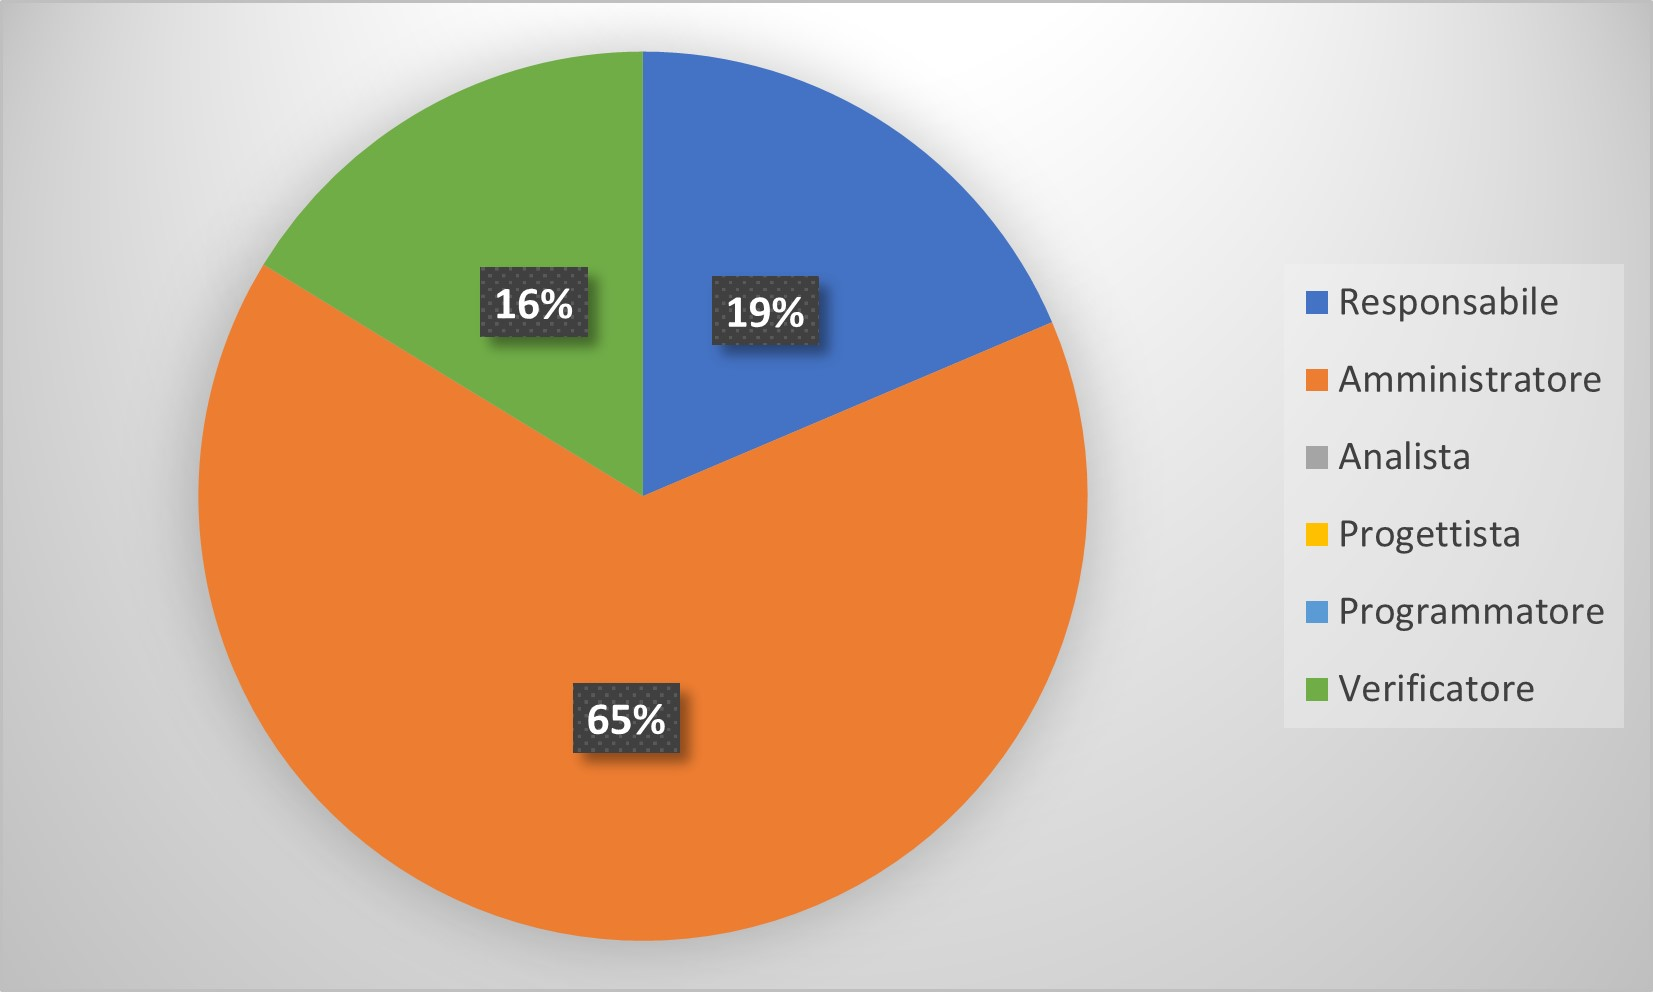
\includegraphics[width=1.0\textwidth]{Torta1.2.jpg}
    \caption{Grafico a torta della distribuzione dei costi} 
\end{figure}

\newpage
\subsection{Secondo periodo}

In questa fase i ruoli da ricoprire per portare a termine gli obiettivi
pianificati sono:
\begin{itemize}
    \item \textit{Responsabile}
    \item \textit{Amministratore}
    \item \textit{Analista}
    \item \textit{Verificatore}
\end{itemize}

\subsubsection{Preventivo orario}

\begin{table}[!ht]
    \centering
    \begin{tabular}{|l|c|c|c|c|c|c|c|}
    \hline
    \textbf{Membro} & \multicolumn{1}{l|}{\textbf{RE}} & \multicolumn{1}{l|}{\textbf{AM}} & \multicolumn{1}{l|}{\textbf{AN}} & \multicolumn{1}{l|}{\textbf{PT}} & \multicolumn{1}{l|}{\textbf{PR}} & \multicolumn{1}{l|}{\textbf{VE}} & \multicolumn{1}{l|}{\textbf{Totale ore persona}} \\ \hline
    \textit{Marco Mazzucato}  & - & 2  & 2  & - & - & 3  & 7  \\ \hline
    \textit{Marco Mamprin}    & - & 2  & 1  & - & - & 2  & 5  \\ \hline
    \textit{Marko Vukovic}    & - & -  & 4  & - & - & 3  & 7  \\ \hline
    \textit{Mattia Zanellato} & - & -  & 4  & - & - & 3  & 7  \\ \hline
    \textit{Emanuele Pase}    & - & -  & 4  & - & - & 3  & 7  \\ \hline
    \textit{Riccardo Contin}  & 4 & -  & 3  & - & - & 1  & 8  \\ \hline
    \textit{Lorenzo Onelia}   & - & 2  & 2  & - & - & 3  & 7  \\ \hline
    \textbf{Totale ore ruolo} & 4 & 6  & 20 & - & - & 18 & 48 \\ \hline
    \end{tabular}
    \caption{Distribuzione delle ore per la seconda milestone}
\end{table}

\begin{figure}[!ht]
    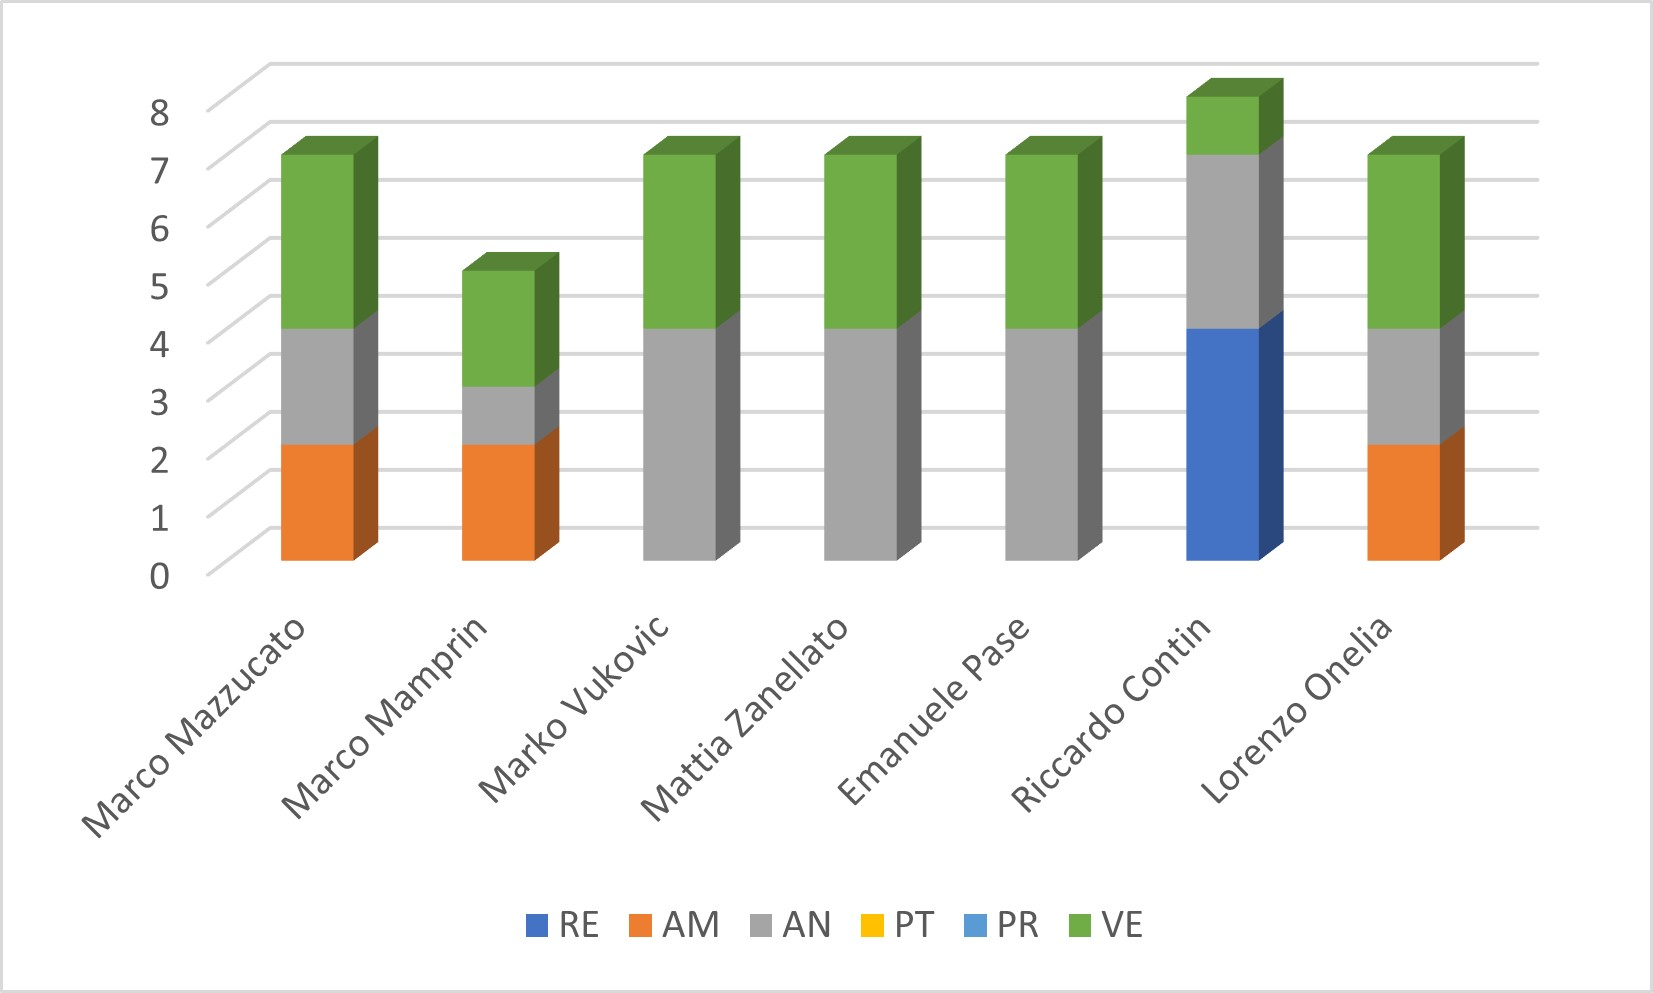
\includegraphics[width=1.0\textwidth]{Istogramma2.jpg}
    \caption{Istogramma della distribuzione delle ore} 
\end{figure}

\begin{figure}[!ht]
    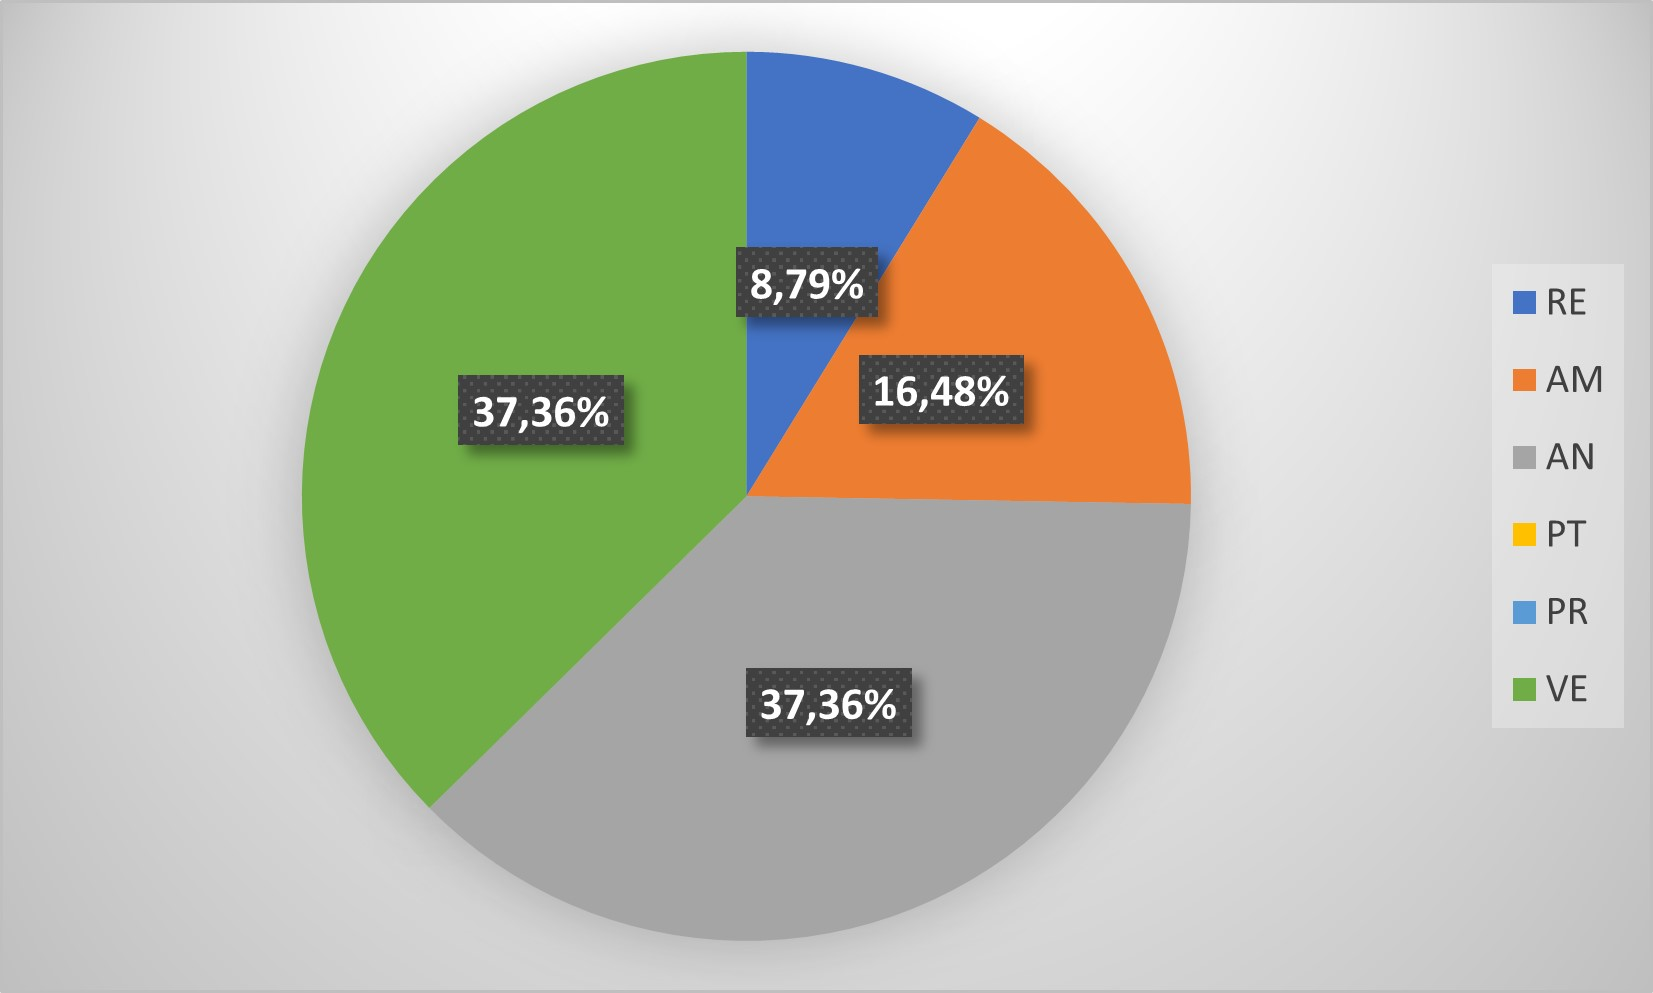
\includegraphics[width=1.0\textwidth]{Torta2.1.jpg}
    \caption{Grafico a torta della distribuzione delle ore} 
\end{figure}

\newpage
\subsubsection{Preventivo economico}

\begin{table}[!ht]
    \centering
    \begin{tabular}{|l|c|c|}
    \hline
    \textbf{Ruolo} & \multicolumn{1}{l|}{\textbf{Ore}} & \multicolumn{1}{l|}{\textbf{Costo (€)}} \\ \hline
    \textit{Responsabile} & 4 & 120 \\ \hline
    \textit{Amministratore} & 6 & 120 \\ \hline
    \textit{Analista} & 19 & 500 \\ \hline
    \textit{Progettista} & - & - \\ \hline
    \textit{Programmatore} & - & - \\ \hline
    \textit{Verificatore} & 17 & 270 \\ \hline
    \textbf{Totale} & 46 & 1010 \\ \hline
    \end{tabular}
    \caption{Prospetto dei costi per la seconda milestone}
\end{table}

\begin{figure}[!ht]
    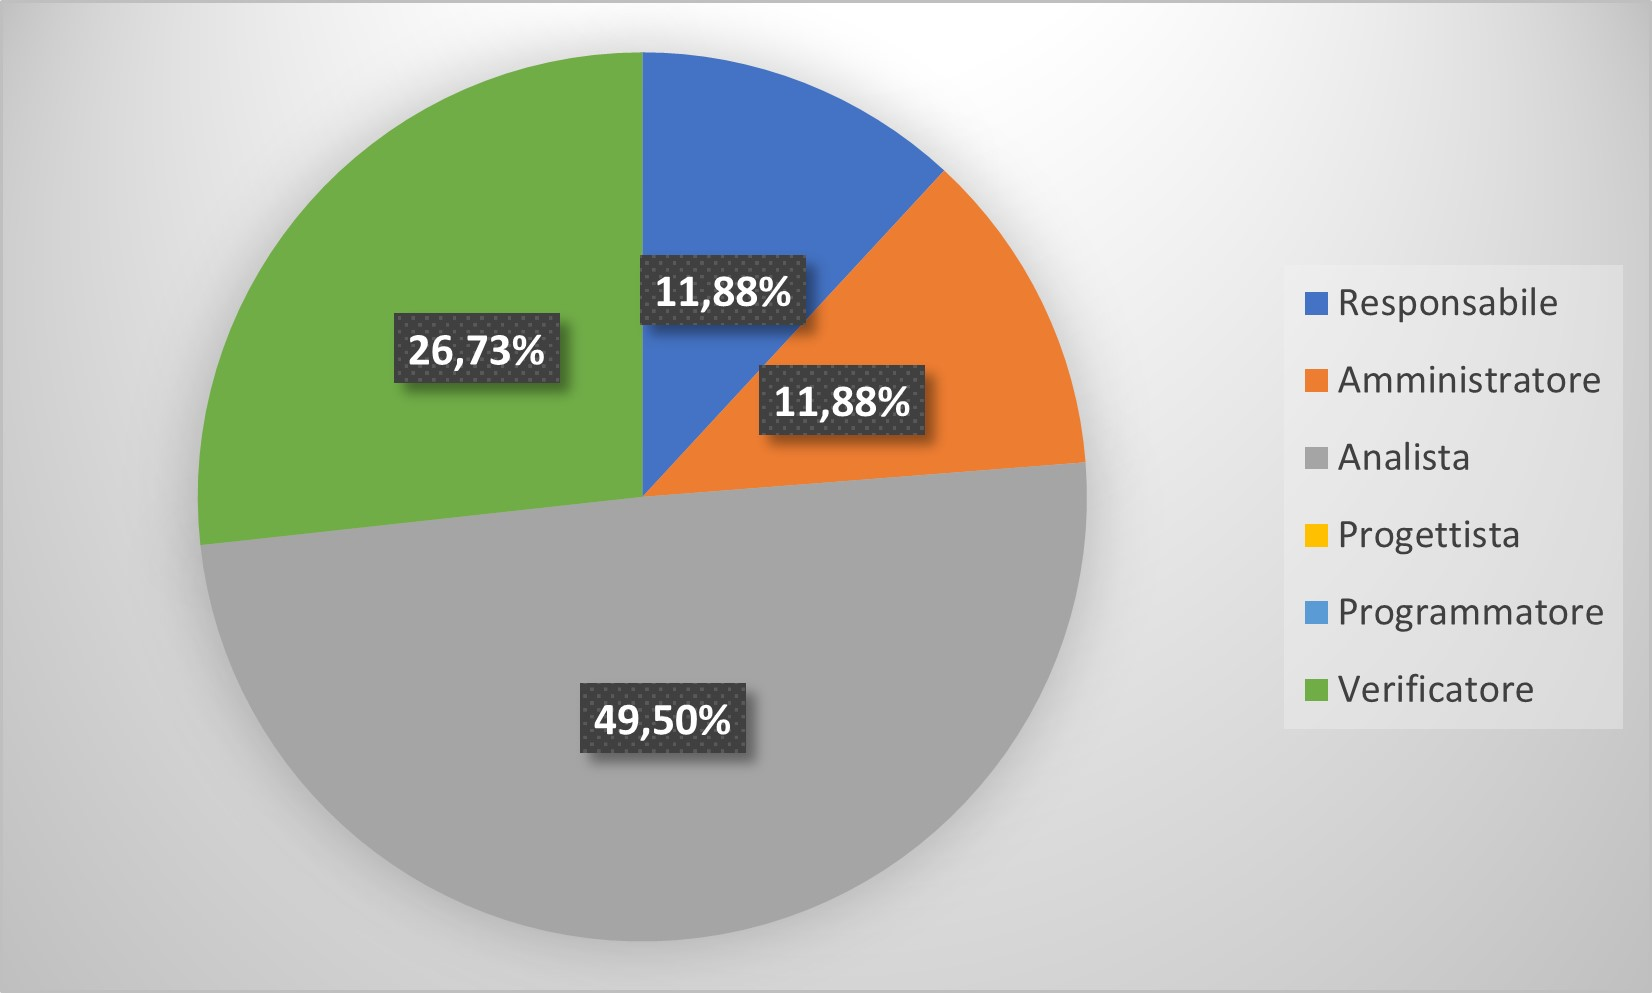
\includegraphics[width=1.0\textwidth]{Torta2.2.jpg}
    \caption{Grafico a torta della distribuzione dei costi} 
\end{figure}

\newpage
\subsection{Terzo periodo}

\section{Verso la PB}

\section{Verso la CA}
  \chapter{Consuntivo}

\section{Verso la RTB}

\subsection{Primo periodo}

\subsubsection{Consuntivo orario}
\begin{table}[!ht]
    \centering
    \begin{tabular}{|l|c|c|c|c|c|c|c|}
    \hline
    \textbf{Membro} & \multicolumn{1}{c|}{\textbf{RE}} & \multicolumn{1}{c|}{\textbf{AM}} & \multicolumn{1}{c|}{\textbf{AN}} & \multicolumn{1}{c|}{\textbf{PT}} & \multicolumn{1}{c|}{\textbf{PR}} & \multicolumn{1}{c|}{\textbf{VE}} & \multicolumn{1}{c|}{\textbf{Totale ore persona}} \\ \hline
    \textit{Marco Mazzucato}  & 2 (+1) & 3        & - & - & - & 1        & 6 (+1)   \\ \hline
    \textit{Marco Mamprin}    & -      & 3 (-1)   & - & - & - & 1 (+0.5) & 4 (-0.5) \\ \hline
    \textit{Marko Vukovic}    & 2      & 3        & - & - & - & 1        & 6        \\ \hline
    \textit{Mattia Zanellato} & -      & 3 (-1.5) & - & - & - & 1 (+1.5) & 4        \\ \hline
    \textit{Emanuele Pase}    & -      & 3 (-0.5) & - & - & - & 1        & 4 (-0.5) \\ \hline
    \textit{Riccardo Contin}  & -      & 3        & - & - & - & 1        & 4        \\ \hline
    \textit{Lorenzo Onelia}   & -      & 3 (-0.5) & - & - & - & 1 (+1)   & 4 (+0.5) \\ \hline
    \textbf{Totale ore ruolo} & 4 (+1) & 21 (-3.5)& - & - & - & 7 (+3)   & 32 (+0.5)\\ \hline
    \end{tabular}
    \caption{Distribuzione delle ore per la prima milestone}
\end{table}

\begin{table}[!ht]
    \centering
    \begin{tabular}{|l|c|c|c|c|c|c|c|}
    \hline
    \textbf{Membro} & \multicolumn{1}{l|}{\textbf{RE}} & \multicolumn{1}{l|}{\textbf{AM}} & \multicolumn{1}{l|}{\textbf{AN}} & \multicolumn{1}{l|}{\textbf{PT}} & \multicolumn{1}{l|}{\textbf{PR}} & \multicolumn{1}{l|}{\textbf{VE}} & \multicolumn{1}{l|}{\textbf{Totale ore persona}} \\ \hline
    \textit{Marco Mazzucato}  & 6  & 5   & 5  & 23  & 24 & 25   & 88   \\ \hline
    \textit{Marco Mamprin}    & 9  & 6   & 5  & 23  & 24 & 24.5 & 91.5 \\ \hline
    \textit{Marko Vukovic}    & 7  & 5   & 5  & 23  & 24 & 25   & 89   \\ \hline
    \textit{Mattia Zanellato} & 9  & 6.5 & 5  & 23  & 24 & 23.5 & 91   \\ \hline
    \textit{Emanuele Pase}    & 9  & 5.5 & 5  & 23  & 24 & 25   & 91.5 \\ \hline
    \textit{Riccardo Contin}  & 9  & 5   & 5  & 23  & 24 & 25   & 91   \\ \hline
    \textit{Lorenzo Onelia}   & 9  & 5.5 & 5  & 23  & 24 & 24   & 90.5 \\ \hline
    \textbf{Totale ore ruolo} & 58 & 38.5& 35 & 161 & 168& 172  & 632.5\\ \hline
    \end{tabular}
    \caption{Ore rimaste dopo la prima milestone}
\end{table}

\subsubsection{Consuntivo economico}

\begin{table}[!ht]
    \centering
    \begin{tabular}{|l|c|c|}
    \hline
    \textbf{Ruolo} & \multicolumn{1}{l|}{\textbf{Ore}} & \multicolumn{1}{l|}{\textbf{Costo (€)}} \\ \hline
    \textit{Responsabile}      & 4 (+1)    & 120 (+30) \\ \hline
    \textit{Amministratore}    & 21 (-3.5) & 420 (-70) \\ \hline
    \textit{Analista}          & -         & -         \\ \hline
    \textit{Progettista}       & -         & -         \\ \hline
    \textit{Programmatore}     & -         & -         \\ \hline
    \textit{Verificatore}      & 7 (+3)    & 105 (+45) \\ \hline
    \textbf{Totale Preventivo} & 32        & 645       \\ \hline
    \textbf{Totale Consuntivo} & 32.5      & 650       \\ \hline
    \textbf{Differenza}        & +0.5      & +5       \\ \hline
    \end{tabular}
    \caption{Consuntivo dei costi per la prima milestone}
\end{table}

\subsubsection{Conclusioni}
Dal consuntivo si può dedurre che il gruppo è stato quasi in linea con il preventivo di periodo.
L'unica differenza è stata che sono servite meno ore di \textit{Amministratore} e più
ore di \textit{Responsabile} e \textit{Verificatore}. Questo ha portato a una spesa maggiore di 5€ per un
complessivo di 650€ a fronte dei 645€ previsti.
In conclusione il budget rimanente è di \num{12510}€.



\subsection{Secondo periodo}

\subsubsection{Consuntivo orario}
\begin{table}[!ht]
    \centering
    \begin{tabular}{|l|c|c|c|c|c|c|c|}
    \hline
    \textbf{Membro} & \multicolumn{1}{c|}{\textbf{RE}} & \multicolumn{1}{c|}{\textbf{AM}} & \multicolumn{1}{c|}{\textbf{AN}} & \multicolumn{1}{c|}{\textbf{PT}} & \multicolumn{1}{c|}{\textbf{PR}} & \multicolumn{1}{c|}{\textbf{VE}} & \multicolumn{1}{c|}{\textbf{Totale ore persona}} \\ \hline
    \textit{Marco Mazzucato}  & -      & 2            & 2          & - & - & 2 (-1)        & 6 (-1)         \\ \hline
    \textit{Marco Mamprin}    & -      & 2            & 1 (-0.5)   & - & - & 2 (-1)        & 5 (-1.5)       \\ \hline
    \textit{Marko Vukovic}    & -      & 1.5          & 3 (-1)     & - & - & 3             & 7.5 (-1)       \\ \hline
    \textit{Mattia Zanellato} & -      & -            & 3          & - & - & 3 (-0.5)      & 6 (-0.5)       \\ \hline
    \textit{Emanuele Pase}    & -      & -            & 3          & - & - & 3 (-0.5)      & 6 (-0.5)       \\ \hline
    \textit{Riccardo Contin}  & 4      & -            & 3 (-1)     & - & - & 1 (+0.5)      & 8 (-0.5)       \\ \hline
    \textit{Lorenzo Onelia}   & -      & 2 (-2)       & 2 (-1)     & - & - & 3 (+0.5)      & 7 (-2.5)       \\ \hline
    \textbf{Totale ore ruolo} & 4      & 7.5 (-2)     & 17 (-3.5)  & - & - & 17 (-2)       & 45.5 (-7.5)    \\ \hline
    \end{tabular}
    \caption{Distribuzione delle ore per la seconda milestone}
\end{table}

\begin{table}[!ht]
    \centering
    \begin{tabular}{|l|c|c|c|c|c|c|c|}
    \hline
    \textbf{Membro} & \multicolumn{1}{l|}{\textbf{RE}} & \multicolumn{1}{l|}{\textbf{AM}} & \multicolumn{1}{l|}{\textbf{AN}} & \multicolumn{1}{l|}{\textbf{PT}} & \multicolumn{1}{l|}{\textbf{PR}} & \multicolumn{1}{l|}{\textbf{VE}} & \multicolumn{1}{l|}{\textbf{Totale ore persona}} \\ \hline
    \textit{Marco Mazzucato}  & 6  & 3    & 3    & 23  & 24 & 24     & 83     \\ \hline
    \textit{Marco Mamprin}    & 9  & 4    & 4.5  & 23  & 24 & 23.5   & 88     \\ \hline
    \textit{Marko Vukovic}    & 7  & 3.5  & 3    & 23  & 24 & 22     & 82.5   \\ \hline
    \textit{Mattia Zanellato} & 9  & 6.5  & 2    & 23  & 24 & 21     & 85.5   \\ \hline
    \textit{Emanuele Pase}    & 9  & 5.5  & 2    & 23  & 24 & 22.5   & 86     \\ \hline
    \textit{Riccardo Contin}  & 5  & 5    & 3    & 23  & 24 & 23.5   & 83.5   \\ \hline
    \textit{Lorenzo Onelia}   & 9  & 5.5  & 4    & 23  & 24 & 20.5   & 86     \\ \hline
    \textbf{Totale ore ruolo} & 54 & 33   & 21.5 & 161 & 168& 157    & 594.5  \\ \hline
    \end{tabular}
    \caption{Ore rimaste dopo la seconda milestone}
\end{table}

\subsubsection{Consuntivo economico}

\begin{table}[!ht]
    \centering
    \begin{tabular}{|l|c|c|}
    \hline
    \textbf{Ruolo} & \multicolumn{1}{l|}{\textbf{Ore}} & \multicolumn{1}{l|}{\textbf{Costo (€)}} \\ \hline
    \textit{Responsabile}      & 4         & 120         \\ \hline
    \textit{Amministratore}    & 7.5 (-2)  & 150 (-40)   \\ \hline
    \textit{Analista}          & 17(-3.5)  & 425 (-87.5) \\ \hline
    \textit{Progettista}       & -         & -           \\ \hline
    \textit{Programmatore}     & -         & -           \\ \hline
    \textit{Verificatore}      & 17 (-2)   & 255 (-30)   \\ \hline
    \textbf{Totale Preventivo} & 45.5      & 950         \\ \hline
    \textbf{Totale Consuntivo} & 38        & 792.5       \\ \hline
    \textbf{Differenza}        & -7.5      & -157.5      \\ \hline
    \end{tabular}
    \caption{Consuntivo dei costi per la seconda milestone}
\end{table}

\subsubsection{Conclusioni}
Come si può notare dal consuntivo il gruppo non è riuscito a rimanere in linea con quanto preventivato.
\\Le differenze dal preventivo riguardano i ruoli di \textit{Amministratore} (-2 ore svolte), \textit{Analista} (-3.5 ore svolte) e \textit{Verificatore} (-2 ore svolte).
Questo ha portato ad una riduzione della spesa totale preventivata di 157.5€ e una riduzione delle ore produttive pari a 7.5. 
\\Tra le cause della discrepanza tra quanto preventivato e quanto consuntivato possiamo individuare:
    \begin{itemize}
        \item L'indisponibilità del proponente ad un incontro nel periodo festivo;
        \item La presenza di festività che hanno rallentato l'avanzamento dei lavori più di quanto previsto;
        \item L'errata stima di disponibilità oraria di alcuni membri del gruppo.
    \end{itemize}
Per migliorare la prescisione dei prossimi preventivi il gruppo ha deciso di preventivare solamente ore che con molta probabilità verranno svolte,
preferendo comunque aggiungere ore al consuntivo invece che toglierle.
\\Il budget rimanente è di \num{11717,5}€.


\subsection{Terzo periodo}

\section{Verso la PB}

\section{Verso la CA}
  \chapter{Organigramma}
  \chapter{Mitigazione dei Rischi}

\section{Rischi legati alle persone}

\begin{table}[H]
    \centering
    \begin{tabular}{|p{2cm}|p{10cm}|}
    \hline
    \multicolumn{2}{|c|}{\textbf{Disponibilità}} \\ \hline
    \multicolumn{1}{|l|}{\textit{Descrizione}} & Il gruppo si è imbattuto in fasi temporali in cui i membri sono stati più o meno attivi in base agli altri impegni universitari. \\ \hline
    \multicolumn{1}{|l|}{\textit{Mitigazione}} & In alcune fasi uno o più membri non sono riusciti a rispettare le precauzioni prese evidenziando alcuni problemi a livello organizzativo, questo si può vedere dalle differenze tra preventivo e consuntivo. Per risolvere questa difficoltà il gruppo ha iniziato a dare maggior importanza alla fase di preventivazione delle ore in modo da essere il più possibile coerenti con le effettive disponibilità dei membri. \\ \hline
    \end{tabular}
\end{table}

\begin{table}[H]
    \centering
    \begin{tabular}{|p{2cm}|p{10cm}|}
    \hline
    \multicolumn{2}{|c|}{\textbf{Problemi interpersonali}} \\ \hline
    \multicolumn{1}{|l|}{\textit{Descrizione}} & All'inizio i membri del gruppo non si conoscevano tra di loro e questo avrebbe potuto provocare incomprensioni interne. \\ \hline
    \multicolumn{1}{|l|}{\textit{Mitigazione}} & Non verificato. Le precauzioni prese sono state sufficienti e di conseguenza non è stato necessario applicare il piano di contingenza. \\ \hline
    \end{tabular}
\end{table}

\begin{table}[H]
    \centering
    \begin{tabular}{|p{2cm}|p{10cm}|}
    \hline
    \multicolumn{2}{|c|}{\textbf{Mancanza di esperienza personale}} \\ \hline
    \multicolumn{1}{|l|}{\textit{Descrizione}} & La poca esperienza dei membri all'interno di un progetto vasto e complesso ha portato ad alcune situazioni di difficoltà. \\ \hline
    \multicolumn{1}{|l|}{\textit{Mitigazione}} & All'interno del gruppo è presente uno spirito di collaborazione che ha permesso aiuti reciproci in situazioni di difficoltà. In questo modo dove un membro si è trovato in difficoltà c'è sempre stato un altro membro pronto a supportarlo al fine di risolvere le difficoltà insieme. Sono state quindi rispettate le precauzioni e, laddove le difficoltà sono risultate maggiori, i membri hanno seguito il piano di contingenza \\ \hline
    \end{tabular}
\end{table}



\section{Rischi legati all'organizzazione}

\begin{table}[H]
    \centering
    \begin{tabular}{|p{2cm}|p{10cm}|}
    \hline
    \multicolumn{2}{|c|}{\textbf{Scarsa pianificazione}} \\ \hline
    \multicolumn{1}{|l|}{\textit{Descrizione}} & La pianificazione di un progetto di queste dimensioni risulta difficile, ancor di più con scarsa esperienza in merito. Si è visto infatti che più di una volta il consuntivo è risultato lontano dal preventivo per quanto riguarda le tempistiche. \\ \hline
    \multicolumn{1}{|l|}{\textit{Mitigazione}} & Come evidenziato in precedenza ci sono state alcune difficoltà a livello di organizzazione. Le precauzioni prese hanno ridotto la gravità dei problemi creati da pianificazioni errate e il piano di contingenza ha fortemente contribuito ad aiutare il gruppo a dare maggior importanza alla fase di preventivazione. \\ \hline
    \end{tabular}
\end{table}



\section{Rischi legati alle tecnologie e agli strumenti}

\begin{table}[H]
    \centering
    \begin{tabular}{|p{2cm}|p{10cm}|}
    \hline
    \multicolumn{2}{|c|}{\textbf{Strumenti sconosciuti}} \\ \hline
    \multicolumn{1}{|l|}{\textit{Descrizione}} & La buona riuscita di un progetto prevede l'utilizzo di strumenti non sempre conosciuti. \\ \hline
    \multicolumn{1}{|l|}{\textit{Mitigazione}} & Le precauzioni prese sono state sufficienti in quanto l'utilizzo di un nuovo strumento è sempre stato anticipato da una discussione e da un'analisi da parte del gruppo. Dopo una prima visione di gruppo ogni membro si è impegnato nello studio individuale dei vari strumenti che sono stati utilizzati. \\ \hline
    \end{tabular}
\end{table}

\begin{table}[H]
    \centering
    \begin{tabular}{|p{2cm}|p{10cm}|}
    \hline
    \multicolumn{2}{|c|}{\textbf{Tecnologie sconosciute}} \\ \hline
    \multicolumn{1}{|l|}{\textit{Descrizione}} & La codifica del software richiede chiaramente la conoscenza di tecnologie specifiche, non sempre conosciute. \\ \hline
    \multicolumn{1}{|l|}{\textit{Mitigazione}} & Le precauzioni prese sono state efficaci in quanto la discussione di gruppo ed il successivo studio individuale hanno portato a buoni risultati. Inoltre è stato organizzato un incontro con un'esperta di \textit{Zucchetti S.p.A.} al fine di migliorare le conoscenze riguardo la libreria \textit{D3.js}. \\ \hline
    \end{tabular}
\end{table}



\section{Rischi legati ai requisiti}

\begin{table}[H]
    \centering
    \begin{tabular}{|p{2cm}|p{10cm}|}
    \hline
    \multicolumn{2}{|c|}{\textbf{Analisi dei requisiti incompleta}} \\ \hline
    \multicolumn{1}{|l|}{\textit{Descrizione}} & L'\textit{Analisi dei Requisiti} è parte fondamentale per la realizzazione del prodotto finale, per questo è necessario che sia completa ed esaustiva. \\ \hline
    \multicolumn{1}{|l|}{\textit{Mitigazione}} & L'\textit{Analisi dei Requisiti} è stata realizzata approfondendo il più possibile i casi d'uso e i requisiti anche grazie ad un confronto diretto con il proponente del progetto in modo che fosse ben chiaro come dovrà essere il prodotto finale. Questo ha permesso al gruppo di effettuare, fino a questo momento, un'analisi soddisfacente. Sono state quindi rispettate le precauzioni. \\ \hline
    \end{tabular}
\end{table}

\end{document}
